In this section the results based on the performed user tests and user evaluation are presented. There were 9 test users, whereof 2 were female and 7 were male. All of them were in their 20s and studying at KTH.

\section{Effectiveness and Efficiency}

\subsection{Time and Commands}
Table \ref{fig:avg_data} declares the average time in seconds and the average amount of commands it took for the users to complete each version of the game. The data shows that it takes 38\% more time and almost double the amount of commands (99.67\% more) to complete the speech version when compared to the text version.

\begin{table}[ht]
  \centering
  \begin{tabular}{l|ccc}
    \toprule
     & Speech &   & Text\\
    \midrule
    Avg. Time & 445.22 &   & 310.22\\
    Avg. Commands & 64.33 &   & 31.22\\
    \bottomrule
  \end{tabular}
  \caption{Average time and commands used to complete the game}\label{fig:avg_data}
\end{table}

This can also be seen in figure \ref{ideal_cmd}, where the average amount of commands used in each version of the game are compared to the ideal number of commands for each version. The ideal takes into consideration a realistic first playthrough of the game, where the player does not ``magically know'' what items are in each room. Therefore, when entering a room, the command “search room” was used to get the list of items located in the room. No items in the rooms were checked, just taken and used, unless the puzzle required looking at specific items (e.g. searching the desk to find the key). In figure \ref{ideal_cmd} it is also shown that the ideal number of commands are about the same for both versions of the game, making the difference in average number of commands even more significant.

\begin{figure}[ht]
  \centering
  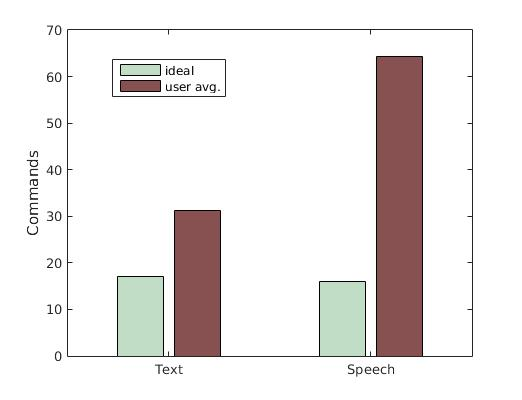
\includegraphics[width=0.8\textwidth]{images/ideal_cmd.jpg}
  \caption{Average amount of commands used compared to the ideal}\label{ideal_cmd}
\end{figure}

\subsection{English Confidence} \label{sec:eng_con}
Each user rated their spoken and written English on a scale 1-5, where 1 equals ``not good'' and 5 equals ``fluent''. The users were divided into groups based on their estimated English level and the average amount of commands, time played and usability score were calculated for each group.

Figure \ref{eng_cmd} shows the average amount of commands used to complete the different versions of the game taking into consideration the English levels of the users. Regarding the speech version, a decrease in amount of commands can be seen as the English level increases. However, there is not much difference between the English levels when looking at the text version. In general less commands were used in the text version for all English levels.

\begin{figure}[ht]
  \centering
  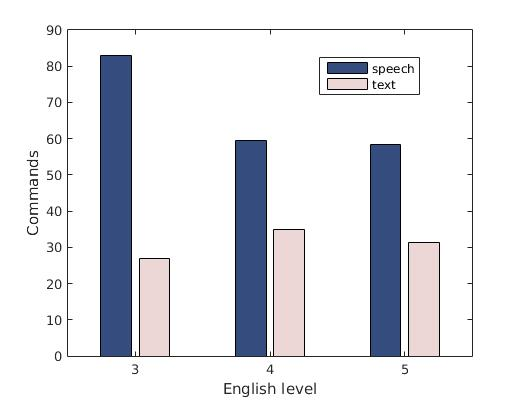
\includegraphics[width=0.8\textwidth]{images/english_cmd.jpg}
  \caption{Average amount of commands used per English level-group}\label{eng_cmd}
\end{figure}

Figure \ref{eng_time} shows the average time to complete the different versions of the game taking into consideration the English levels of the users. Regarding the speech version a decrease in time can be seen as the English level is increased. In general it took more time to complete the speech version than the text version except for users of English level 4, where the speech version took less time to complete.

\begin{figure}[H]
  \centering
  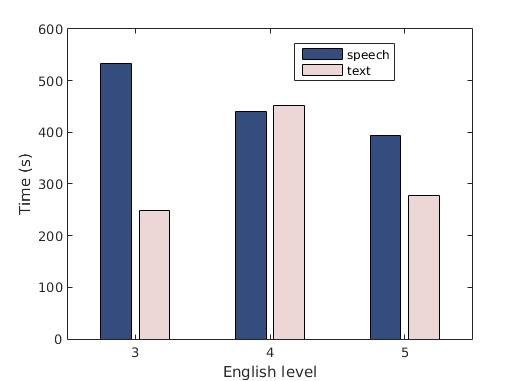
\includegraphics[width=0.8\textwidth]{images/english_time.jpg}
  \caption{Average time to complete the game per English level-group}\label{eng_time}
\end{figure}

Figure \ref{eng_score} shows the average SUS score for each version of the game per English level. Looking at the speech version the score increases as the English level increases. The text version shows no such correlation. In general the text version have higher SUS scores for each English level.

\begin{figure}[H]
  \centering
  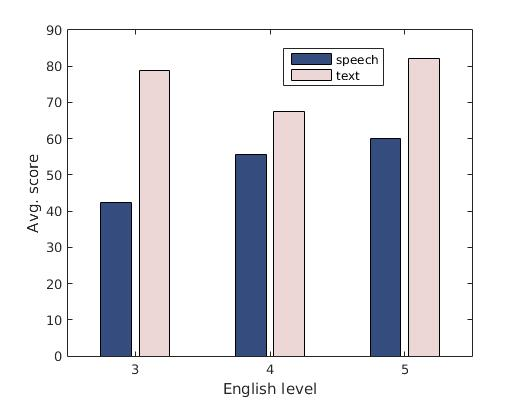
\includegraphics[width=0.8\textwidth]{images/english_score.jpg}
  \caption{Average score based on the SUS per English level-group}\label{eng_score}
\end{figure}

%\subsection{User Former Experience}
%\newpage
\section{Satisfaction (SUS)} 
The average total usability score based on the SUS for each version can be seen in table \ref{tot_score}. The text version got a significantly higher usability score than the speech version.

\begin{table}[ht]
  \centering
  \begin{tabular}{ccc}
    \toprule
    Speech &   & Text\\
    \midrule
    54.17 &   & 78.06\\
    \bottomrule
  \end{tabular}
  \caption{Average score based on the SUS}\label{tot_score}
\end{table}
